% !TEX root = NSF_SuperCDMS_SNOLAB_OPS.tex
\section{SuperCDMS SNOLAB (2 pages)}
\label{sec:snolab}

\begin{figure}
\centering
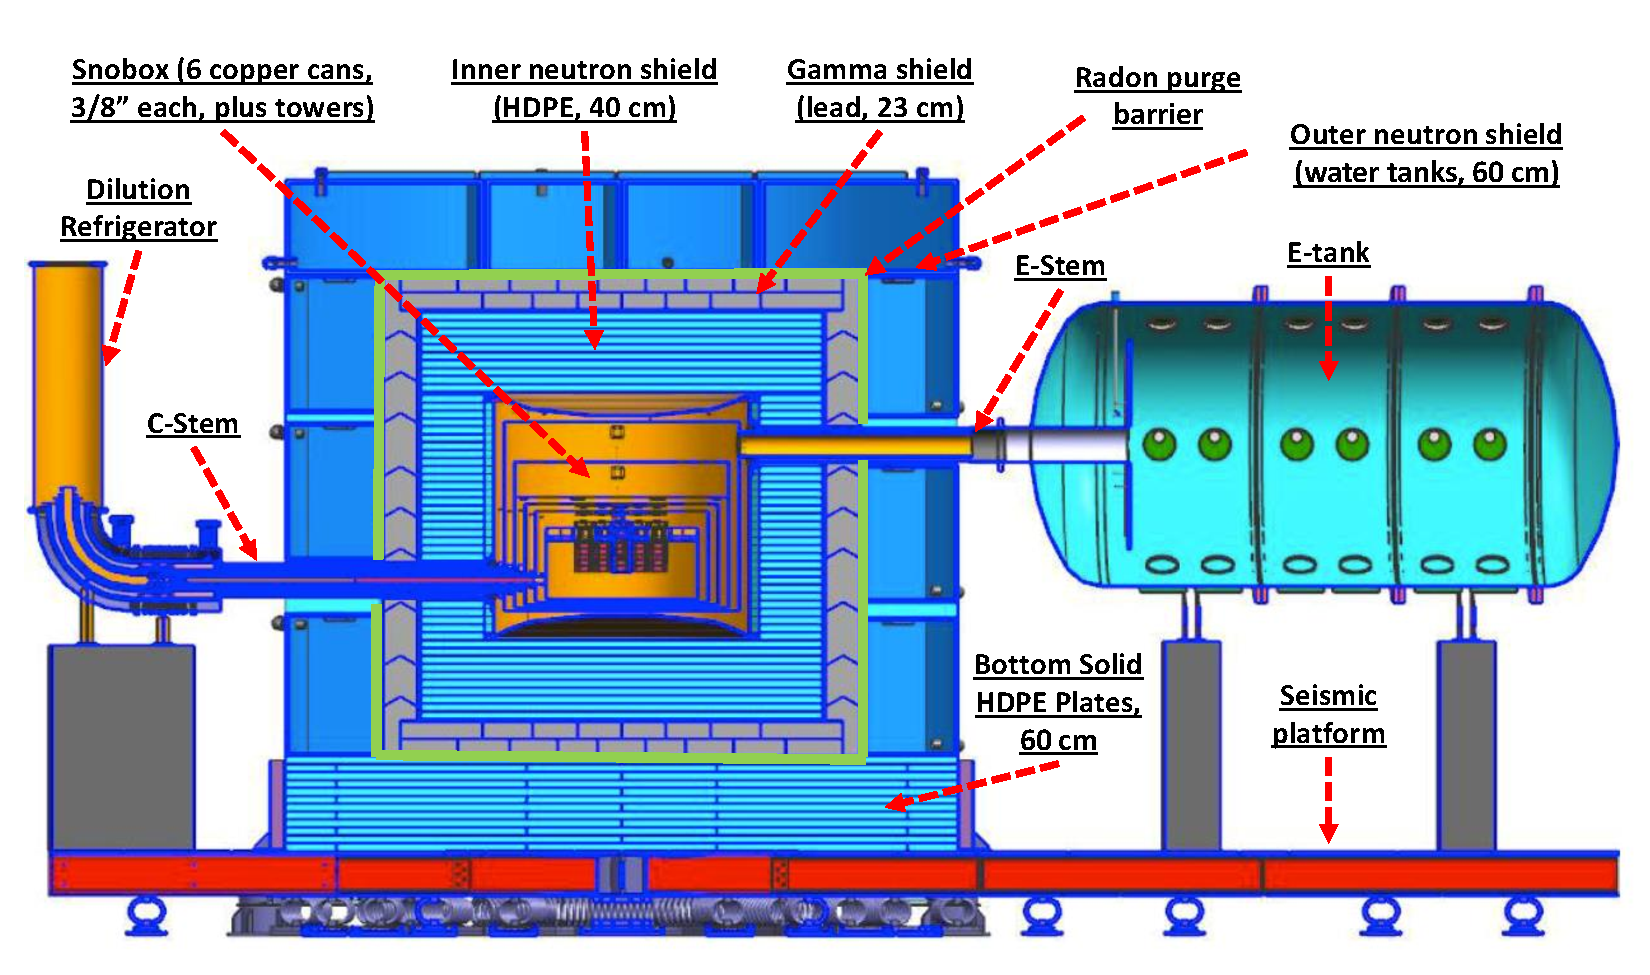
\includegraphics[width=0.8\textwidth]{Figures/f02_SuperCDMS_Schematic.pdf}
\caption{\footnotesize Schematic of the SuperCDMS SNOLAB experiment. The detectors reside within the inner can of the copper cryostat, and are shielded from the environment. A gamma shield protects from external gamma-rays and the inner polyethylene layers serve to absorb radiogenic neutrons emitted from the cryostat and gamma shield. The outer water tanks provide protection from external neutrons. The assembly rests on top of a seismic platform to provide isolation from seismic events. }
\label{fig:SCDMS_schematic}
\end{figure}

\begin{table}
\centering
\small
\begin{tabular}{  l  c  c  c  c } \hline
&\multicolumn{2}{c}{iZIP} & \multicolumn{2}{c}{HV}\\ 
&  Ge & Si    & Ge & Si \\ \hline
Number of detectors & 10 & 2 & 8 & 4\\
Total exposure (kg\(\cdot\)yr) & 56  & 4.8 & 44 & 9.6 \\
Phonon resolution (eV) & 50 & 25 & 10 & 5\\
Ionization resolution (eV) & 100 & 110 & -- & -- \\
Voltage Bias (V) & 6 & 8 & 100 & 100\\ \hline
\end{tabular}
\caption{The anticipated exposures and detector parameters for the SuperCDMS SNOLAB experiment. The exposures are based on 5 years of operation (from 2020--2024) with an 80\% live time. The quoted phonon energy resolutions represent the r.m.s.\ values of the total measured quantity (\textit{i.e.}, combining all active sensors). The quoted ionization resolution is derived from the readout electronics equivalent noise charge value of 33\textit{e} and represents the r.m.s.\ energy resolution of a single channel for electron recoils.}
\label{tab:ExpOperations}
\vspace{-20pt}
\end{table}


The SuperCDMS SNOLAB experiment will be a next-generation direct dark matter search specifically designed to explore the low mass ($<$ 10 GeV/c$^{2}$) dark matter region, with ultimate sensitivity to dark matter-nucleon cross sections where solar neutrino-nucleus scattering becomes significant (the so-called “neutrino floor”). The SuperCDMS SNOLAB G2 Project is being designed to provide a shielded, ultra-low-background cryostat capable of housing up to 31 towers of solid state cryogenic detectors.% operating at temperatures in the 15--40 mK range. 
The SuperCDMS SNOLAB Project baseline is outlined in Table~\ref{tab:ExpOperations}. The experiment will include a mixture of detectors composed of cylindrical germanium (Ge) and silicon (Si) crystals, 100 mm in diameter and 33.3 mm thick. Each Ge(Si) crystal will have a mass of 1.39(0.61)~kg. The detectors will be stacked into four towers of six detectors. Two towers of detectors will be operated in the ultra-low-energy threshold high-voltage mode (HV), providing the best sensitivity for dark matter masses below 5 GeV/c$^{2}$~\cite{Agnese:2015nto}. An additional two towers of germanium and silicon detectors will be operated in standard (iZIP) mode. These detectors will provide better sensitivity in the 5--10 GeV/c$^{2}$ mass range due to their capability to discriminate between electron-recoil and nuclear-recoil interactions ~\cite{Agnese:2014aze}. The anticipated exposure and detector parameters for SuperCDMS SNOLAB can be found in Table~\ref{tab:ExpOperations}. 

The detector towers will be cooled to ~15--30 mK using a dilution refrigerator and cryocoolers. The cold region of the full experiment, referred to as the SNOBOX, consists of 6 cylindrical copper cans suspended by Kevlar ropes. In the design, the SNOBOX is surrounded by a 40 cm thick layer of polyethylene to moderate and absorb neutrons produced by radiogenic contamination, and to provide a shield from external neutrons. This inner polyethylene layer is surrounded by a 23 cm thick gamma shield made from low-activity lead. The lead shield layer is surrounded by a thin metal shield to block radon (Rn) diffusion into the inner shielding layers. This volume will be purged with boil-off nitrogen gas to reduce the overall Rn levels and the backgrounds caused by prompt Rn daughters. The outermost shield layer consists of polyethylene and water tanks that provide additional shielding from the cavern neutron flux. A schematic of the experiment shield and cryostat layers can be seen in Fig \ref{fig:SCDMS_schematic}. 

The large cryostat and passive shield provide the capability to expand the detector mass to the necessary level that would allow full exploration of the low-mass dark matter parameter space down to dark matter-nucleon cross sections where solar neutrino-nucleus scattering becomes significant. This could be accomplished through a combination of SuperCDMS detector tower upgrades and incorporation of similar detectors from the EURECA collaboration.





